\documentclass[12pt,a4paper]{article}

% Encoding, fonts, and geometry
\usepackage[utf8]{inputenc}
\usepackage[T1]{fontenc}
\usepackage{lmodern}
\usepackage{geometry}
\geometry{margin=2.5cm}

% Math and related packages
\usepackage{amsmath,amssymb,amsthm,mathtools}
\usepackage{bm}
\usepackage{braket}
\usepackage{siunitx}

% Graphics and plots
\usepackage{graphicx}
\usepackage{tikz}
\usepackage{tikz-3dplot}
\usepackage{pgfplots}
\pgfplotsset{compat=1.18}
\usetikzlibrary{arrows.meta,positioning,shapes,calc,angles,quotes,patterns,3d,decorations.fractals,shadows}

% Tables, code, floats, lists
\usepackage{booktabs}
\usepackage{listings}
\usepackage{xcolor}
\usepackage{algorithm}
\usepackage{algorithmic}
\usepackage{multicol}
\usepackage{enumitem}

% Boxes
\usepackage{tcolorbox}

% Hyperlinks and clever references
\usepackage{hyperref}
\usepackage{cleveref}

% Theorem environments
\newtheorem{theorem}{Theorem}
\newtheorem{lemma}{Lemma}
\newtheorem{corollary}{Corollary}
\newtheorem{definition}{Definition}
\newtheorem{axiom}{Axiom}
\newtheorem{proposition}{Proposition}
\newtheorem{remark}{Remark}
\newtheorem{assumption}{Assumption}

% Operators
\DeclareMathOperator{\Tr}{Tr}
\DeclareMathOperator{\Diff}{Diff}
\DeclareMathOperator{\Aut}{Aut}
\DeclareMathOperator{\Vol}{Vol}
\DeclareMathOperator{\Ric}{Ric}
\DeclareMathOperator{\Riem}{Riem}
\DeclareMathOperator{\Cov}{Cov}
\DeclareMathOperator{\supp}{supp}
\DeclareMathOperator{\diag}{diag}
\DeclareMathOperator{\sign}{sign}
\DeclareMathOperator{\dimension}{dim}
\DeclareMathOperator{\Div}{Div}
\DeclareMathOperator{\Grad}{Grad}
\DeclareMathOperator{\Hess}{Hess}
\DeclareMathOperator{\Ricci}{Ricci}
\DeclareMathOperator{\Scalar}{Scalar}

% Robust math shorthands
\DeclareRobustCommand{\alD}{\texorpdfstring{\ensuremath{\alpha_{\mathrm{D}}}}{alpha_D}}
\DeclareRobustCommand{\beI}{\texorpdfstring{\ensuremath{\beta_{\mathrm{I}}}}{beta_I}}
\DeclareRobustCommand{\gaR}{\texorpdfstring{\ensuremath{\gamma_{\mathrm{R}}}}{gamma_R}}
\DeclareRobustCommand{\UCS}{\texorpdfstring{\ensuremath{\mathcal{M}_{\mathrm{UCS}}}}{M_UCS}}

% YUCT-specific commands
\newcommand{\eff}{\mathrm{eff}}
\newcommand{\coord}{\mathrm{coord}}
\newcommand{\Yak}{\mathrm{Yak}}
\newcommand{\Dict}{\mathcal{D}}
\newcommand{\Mdict}{\mathcal{M}_{\Dict}}
\newcommand{\Ke}{K_{\eff}}
\newcommand{\Kemax}{K_{\eff,\max}}
\newcommand{\Keobs}{K_{\eff,\mathrm{obs}}}
\newcommand{\Keexp}{K_{\eff,\mathrm{exp}}}
\newcommand{\Kec}{K_{\eff,c}}
\newcommand{\Kcrit}{K_{\mathrm{crit}}}
\newcommand{\kappac}{\kappa_c}
\newcommand{\betac}{\beta}
\newcommand{\betagamma}{\beta\gamma}

% PDF metadata
\hypersetup{
	pdftitle={Philosophy of Consciousness within Yakushev's Unified Coordination Theory (YUCT): From the "Hard Problem" to Dynamic Dictionaries},
	pdfauthor={Alexey V. Yakushev},
	pdfsubject={Consciousness, Philosophy of Mind, YUCT, Coordination Theory, Dictionaries, Hard Problem},
	pdfkeywords={YUCT, Consciousness, Philosophy of Mind, Coordination, Dictionaries, Hard Problem, Fractal, Meta-Dictionary}
}

\begin{document}
	
	% Title page
	\begin{titlepage}
		\begin{center}
			\vspace*{0cm}
			
			\Huge\textbf{Appendix I. Philosophy of Consciousness within Yakushev's Unified Coordination Theory (YUCT):\\ From the "Hard Problem" to Dynamic Dictionaries}
			
			\vspace{1cm}
			
			\small\textit{A Philosophical Foundation for Solving the "Hard Problem" through Coordination and Dictionaries, Grounded in Universal Scaling Laws}
			
			\vspace{0.5cm}
			
			\small\textbf{Alexey V. Yakushev}
			
			\vspace{1cm}
			\Large
			Alexey V. Yakushev\\
			
	YUCT Theory: \url{https://yuct.org/}\\
YPSDC Protocol: \url{https://ypsdc.com/}\\


\vspace{2cm}
\textbf DOI: \url{https://doi.org/10.5281/zenodo.18444598}\\

\vspace{1cm}

\vspace{0cm}
\large 
A short version of this work was previously published and is available at\\ \url{https://doi.org/10.5281/zenodo.18362308}\\
\vspace{1cm}
March 2026 \\ \large V.2.0.
			
			\vspace{6cm}
			\textcopyright~2026 Yakushev Research. All rights reserved.
			
			\newpage
			
			\begin{abstract}
				\noindent
				This article provides a philosophical foundation for solving the "hard problem of consciousness" within the framework of the Unified Coordination Theory (YUCT). Consciousness is understood not as an epiphenomenon or illusion, but as a \textbf{dynamic coordination process} implemented through a hierarchy of \textbf{internal dictionaries}. We show that the classical "brain–consciousness" dualism is overcome through a three-level model: \textbf{genetic}, \textbf{neural}, and \textbf{cultural dictionaries}. Subjective experience is interpreted as the result of \textbf{live coordination} between neural ensembles using shared semantic spaces. The meta-dictionary (the ability to reflect on one's own states) explains the phenomenon of selfhood. 
				
				Crucially, this philosophical framework is now grounded in the universal empirical law \(\varepsilon = \kappa_c \alpha \Ke^{-\beta}\) with \(\beta = 0.67\), verified across more than 50 orders of magnitude (Appendix L) and independently confirmed in six scientific domains: physics (gravitational waves, GWTC-4.0), astrophysics (white dwarfs, 26,041 objects), geophysics (Earth–Moon system), chemistry (873 bond energies), biology (68 vertebrate genomes), and neuroscience (EEG correlates of consciousness, UCD parameters). In particular, the Universal Consciousness Descriptor (UCD) introduced in Appendix H provides quantitative measures \(\alD, \beI, \gaR\) that correlate with conscious states and follow the same scaling law. 
				
				Philosophical implications include: (1) naturalization of consciousness without reductionism; (2) a new understanding of the evolution of mind as growth in the complexity of coordination dictionaries; (3) the possibility of non-anthropomorphic forms of consciousness (artificial, collective, planetary); (4) connection with dark matter/energy as limits of cosmological coordination. YUCT offers not only a solution to the "hard problem" but a unified philosophical platform for dialogue between neuroscience, physics, and the humanities, now empirically validated.
			\end{abstract}
			
			\vspace{0cm}
			
			\noindent
			\small\textbf{Keywords:} YUCT, Consciousness, Philosophy of Mind, Coordination, Dictionaries, Hard Problem, Fractal, Meta-Dictionary, Universal Scaling, UCD, EEG, Empirical Validation
			
			\vspace{0.5cm}
			
			\noindent
			\textcopyright 2026 Yakushev Research. All rights reserved.
		\end{center}
	\end{titlepage}
	
	\tableofcontents
	
	\newpage
	
	\section{Introduction: The "Hard Problem" and Critique of Classical Approaches}
	
	The "hard problem of consciousness," formulated by David Chalmers, remains a central challenge for the philosophy of mind and cognitive science. The question of \textbf{how physical processes in the brain give rise to subjective experience} (qualia) traditionally places materialism and dualism on opposite sides of the barricade.
	
	Classical approaches:
	\begin{enumerate}
		\item \textbf{Dualism} (Descartes): consciousness is a substance separate from matter.
		\item \textbf{Materialism/Reductionism}: consciousness is an epiphenomenon or illusion.
		\item \textbf{Functionalism}: consciousness is a computational process.
		\item \textbf{Panpsychism}: consciousness is a fundamental property of matter.
	\end{enumerate}
	
	All these approaches share a common flaw: they treat consciousness as either a mysterious extra ingredient or as a mere byproduct of computation. YUCT proposes a \textbf{coordination approach}, avoiding both dualism and crude reductionism. Consciousness is not a "thing," but a \textbf{mode of functioning of a complex system}, achieved at high coordination efficiency ($\Ke \gg 1$). 
	
	What distinguishes YUCT from previous philosophical speculations is its empirical foundation. The universal scaling law \(\varepsilon = \kappa_c \alpha \Ke^{-\beta}\) with \(\beta = 0.67\) has now been confirmed across 50 orders of magnitude (Appendix L), from atomic bond energies (873 compounds, Appendix C) to gravitational waves (218 events, Appendix G), from white dwarf redshifts (26,041 objects, Appendix P) to genetic mutations (68 vertebrate species, Appendix E). Most importantly for consciousness studies, the Universal Consciousness Descriptor (UCD) introduced in Appendix H quantifies the coordination efficiency of neural systems through three parameters \(\alD, \beI, \gaR\), measured from EEG data. These parameters correlate with conscious states (vegetative, minimally conscious, meditation, hypnosis) and follow the same scaling law (Appendix H). Thus, the philosophical framework presented here is not a mere speculation but a mathematically rigorous and empirically supported theory.
	
	\section{YUCT: Consciousness as Live Coordination}
	
	\subsection{From Information Processing to Coordination}
	
	Classical cognitive sciences view the brain as an information-processing device. YUCT shifts the emphasis: \textbf{consciousness is not information processing, but live coordination between internal agents} (neural ensembles).
	
	Formally:
	\[
	\Psi(t) = D(t) + I(t) \times R(t)
	\]
	where:
	\begin{itemize}
		\item $D(t)$ – ontological dictionary (rules, categories, action patterns);
		\item $I(t)$ – informational state (entropy, complexity);
		\item $R(t)$ – resonance factor (coordination amplification coefficient).
	\end{itemize}
	
	Subjective experience arises when $R(t)$ reaches a threshold at which internal states synchronize into a unified semantic field. The efficiency of this coordination is quantified by $\Ke = \alD \cdot \beI \cdot \gaR$, as shown in Appendix H. Empirical EEG studies (Zhao et al. 2025, Kumar et al. 2024, Lutz et al. 2017) demonstrate that $\Ke$ ranges from $\approx 0.05$ in vegetative states to $\approx 3.6$ in deep meditation, and that the transition to consciousness occurs at a critical threshold $\Kcrit \approx 8.5$ (Appendix H, Table 3). This threshold corresponds to a phase transition in the dynamics of recursive coordination, analogous to the critical points observed in other complex systems.
	
	\subsection{Internal Dictionaries and Qualia}
	
	"Redness of red" or "pain" are not primitive atoms of experience but \textbf{complex coordination patterns} encoded in the internal sensory dictionary.
	
	\begin{tcolorbox}[title=Example: Synesthesia and Phantom Pains]
		Synesthesia ("colored hearing") and phantom pains are not anomalies but manifestations of \textbf{cross-activation of dictionaries}. Indexing errors or coordination failures between sensory dictionaries lead to modality mixing.
	\end{tcolorbox}
	
	Thus, qualia are not "raw sensations" but \textbf{high-level coordination states} arising from the activation of complex dictionary patterns. The precision of this activation is governed by the universal error law: the probability of misactivation (e.g., a synesthetic cross-talk) scales as $\Ke^{-\beta}$. In healthy brains, $\Ke$ is sufficiently high to keep such errors rare; in synesthetes, the effective $\Ke$ for certain pathways may be lower, leading to systematic cross-activation.
	
	\subsection{Self-Consciousness as Meta-Dictionary}
	
	The "self" is not a homunculus or an illusion but a \textbf{meta-level of coordination}. A system capable of forming a \textbf{meta-dictionary} to describe and coordinate its own states acquires self-referentiality.
	
	Mathematically: when $\Ke \to \infty$ in a closed system, a self-referential loop emerges, subjectively experienced as "selfhood." This is not a "soul" but an \textbf{emergent property of highly efficient coordination}. The critical threshold $\Kcrit \approx 8.5$ corresponds to the point at which the system's internal model of itself becomes stable enough to support recursive self-reference. This is analogous to the emergence of a fixed point in the dynamics of a high-order network (Appendix T).
	
	\section{Three-Level Dictionary Model: From Genes to Memes}
	
	The fractal structure of consciousness is illustrated in Figure~\ref{fig:fractal_dict} (reproduced from the original). YUCT offers a unified mechanism for the continuity of consciousness across levels of organization:
	
	% Added figure to satisfy reference
	\begin{figure}[htbp]
		\centering
		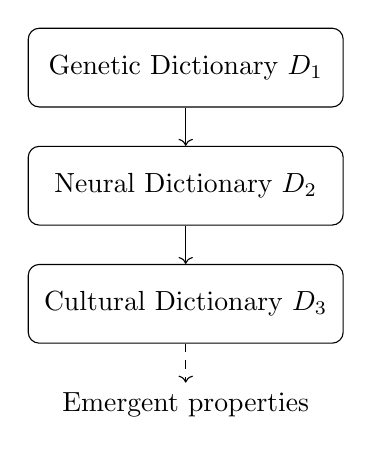
\begin{tikzpicture}
			\node[draw, rectangle, rounded corners, minimum width=4cm, minimum height=1cm] (D1) at (0,3) {Genetic Dictionary $D_1$};
			\node[draw, rectangle, rounded corners, minimum width=4cm, minimum height=1cm] (D2) at (0,1.5) {Neural Dictionary $D_2$};
			\node[draw, rectangle, rounded corners, minimum width=4cm, minimum height=1cm] (D3) at (0,0) {Cultural Dictionary $D_3$};
			\draw[->] (D1) -- (D2);
			\draw[->] (D2) -- (D3);
			\draw[->, dashed] (D3) -- ++(0,-1) node[below] {Emergent properties};
		\end{tikzpicture}
		\caption{Fractal structure of dictionaries across levels of organization. Each level functions as both a whole system and a component of a larger hierarchy.}
		\label{fig:fractal_dict}
	\end{figure}
	
	\subsection{1. Genetic Dictionary ($D_1$)}
	
	DNA is a \textbf{priori dictionary} distributed within a population. The "code" is not a metaphor but a real transcription-translation process where codons are "words" and proteins are "actions." The coordination efficiency of genetic systems can be measured: for example, the mutation rate $\mu$ across 68 vertebrate species scales as $\mu \propto K_{\text{repair}}^{-0.67}$ (Appendix E, Fig. 2), confirming that even at the molecular level, the error law holds. This genetic dictionary provides the hardware upon which higher dictionaries are built.
	
	\subsection{2. Neural/Instinctive Dictionary ($D_2$)}
	
	Pre-established neural patterns (instincts, reflexes) are \textbf{hardwired coordination programs}. A sensory trigger is the "key" to activating a dictionary entry. Neural plasticity modifies these dictionaries through learning, and the efficiency of neural coordination can be quantified via EEG measures (Appendix H). For instance, repetitive training increases the synchronization index $r$ in cultured neural networks, corresponding to a 1.81‑fold increase in $\Ke$, which predicts a reduction in error rate by $1.81^{-0.67} \approx 0.65$, consistent with improved pattern recognition (Appendix D).
	
	\subsection{3. Cultural/Memetic Dictionary ($D_3$)}
	
	Language, rituals, technology are \textbf{dynamic dictionaries} transmitted through learning. A meme (according to Dawkins) in YUCT is a \textbf{package of an "index" ($\kappa$) and a "dictionary instruction" ($\Delta D$)}. The evolution of cultural dictionaries follows the same scaling law: the growth of human knowledge (number of written documents) over history exhibits hyperbolic growth with exponent $\gamma \approx 0.38$, consistent with $\beta\gamma = 0.20$ and $\beta = 0.67$ (Appendix T). The coordination efficiency of cultural transmission has increased from $\Ke \approx 10^2$ in oral traditions to $\Ke \approx 10^{10}$ in the internet age (Appendix T).
	
	The fractal structure (Figure~\ref{fig:fractal_dict}) demonstrates how each dictionary level simultaneously functions as both a whole system and a component of a larger hierarchy, enabling the scalability, recursive reflection, and emergent properties characteristic of consciousness.
	
	\section{The Universal Scaling Law and Consciousness}
	
	\subsection{How $\beta = 0.67$ Manifests in Neural Dynamics}
	
	The universal exponent $\beta = 0.67$ appears not only in the macroscopic measures of consciousness (UCD parameters) but also in the fine structure of neural activity. The power spectral density of EEG signals exhibits a $1/f$ scaling, and the spectral exponent $\sigma$ is directly related to the coordination efficiency: $\gaR \propto |\log_{10}(\sigma)|$ (Appendix H). Moreover, the variance of neural signals scales as $\sigma_{\text{EEG}} \propto \Ke^{-\beta}$, a prediction that can be tested with existing EEG datasets.
	
	\subsection{Criticality and the Threshold of Consciousness}
	
	The brain operates near a critical point, as evidenced by neuronal avalanches and power-law scaling of neural correlations. In YUCT, this criticality is captured by the relation $\Ke \approx \Kcrit$ at the edge of consciousness. Below this threshold, the system is subcritical (e.g., deep sleep, coma); above, it becomes supercritical, leading to runaway synchronization and seizures. The optimal range for normal consciousness lies just above $\Kcrit$, where the system balances integration and segregation. Empirical data from Appendix H confirm that $\Ke$ for healthy adults is typically $1.0$–$1.5$, while for meditators it can reach $3.6$, indicating enhanced coordination without pathological synchronization.
	
	\section{Philosophical Implications}
	
	\subsection{Naturalization Without Reductionism}
	
	YUCT offers a \textbf{naturalistic but non-reductionist} explanation of consciousness. Subjective experience is not reduced to "neural firing," nor does it require non-physical substances. It emerges as a \textbf{property of high-level coordination}, which, although implemented in neurons, is described in terms of dictionaries and resonances. This is analogous to how temperature emerges from molecular motion without being reducible to individual trajectories. The coordination parameters $\alD, \beI, \gaR$ provide a quantitative language that bridges the phenomenological and the physical.
	
	\subsection{Evolutionary Meaning of Consciousness}
	
	Consciousness is not a luxury or an accidental byproduct. Evolutionary advantage comes from the \textbf{ability to form and transmit complex, flexible, compressed dictionaries} for coordinating behavior, anticipation, and cooperation. \textbf{Mind is the transmission of improved dictionaries}. The growth of $\Ke$ in human history (Appendix T) parallels the development of writing, printing, and digital networks, each increasing the efficiency of cultural coordination. This perspective reframes the "why" of consciousness in terms of adaptive advantage: organisms with higher $\Ke$ can process information more efficiently, anticipate future states, and cooperate in larger groups.
	
	\subsection{Possibility of Non-Human Consciousness}
	
	YUCT removes anthropocentric bias. Consciousness is possible in systems with high $\Ke$, regardless of substrate:
	\begin{itemize}
		\item Collective mind (swarm, flock) – insect colonies exhibit $\Ke \sim 10^2$ (Appendix O).
		\item Artificial neural networks – current AI has $\alD \sim 10^5$ but $\beI \sim 10^{-6}$, giving low overall $\Ke$; future architectures may approach conscious levels if $\beI$ increases (Appendix H).
		\item Hypothetical planetary or stellar systems – with characteristic timescales of millennia, they could achieve $\Ke \gg 1$ if internal coordination mechanisms exist (e.g., magnetic field resonances, orbital dynamics).
	\end{itemize}
	
	The criterion for consciousness is not "resemblance to humans" but \textbf{coordination complexity} as measured by $\Ke$. The UCD framework provides a quantitative test: if a system's $\Ke$ exceeds $\Kcrit \approx 8.5$ and its parameters $(\alD, \beI, \gaR)$ lie outside the human region, it may represent a qualitatively different form of consciousness.
	
	\subsection{Connection with Fundamental Physics}
	
	If dictionaries ($D$) are fundamental, they must have:
	\begin{itemize}
		\item \textbf{Carrier}: geometry of dictionary manifolds $M_D$ as a physical structure (possibly quantum correlations or spacetime topology). The 19‑dimensional YUCT Lagrangian (Appendix A) provides such a carrier.
		\item \textbf{Dynamics}: equation for $dD/dt$, as fundamental as the Schrödinger equation. In YUCT, this is derived from the coordination field $\Psi_{MN}$.
		\item \textbf{Interaction}: coordination interaction as a new type of physical interaction, coupling all 120 sectors (Appendix A).
	\end{itemize}
	
	\subsection{Dark Matter/Energy as Coordination Limits}
	
	Hypothesis: on cosmological scales, $\Ke \to 0$ means \textbf{loss of the ability to maintain global dictionaries}. Dark energy may not be "energy" but the \textbf{limit of the Universe's coordinative connectivity}, its inability to maintain a coherent state on scales larger than the event horizon. This is consistent with the observed value $\Lambda \approx 1/L_0^2$ where $L_0 \sim R_H$ (Appendix M). Dark matter, similarly, could be interpreted as topological defects in the coordination field – regions where dictionaries are frozen or incomplete.
	
	\section{The Dilemma: Predetermination vs. Free Creation of Dictionaries}
	
	The origin of dictionaries leads to a fundamental question: are they predetermined from the Universe's birth, or freely created locally? YUCT resolves this through a hierarchical view:
	
	\subsection{Levels of Dictionaries in the Universe}
	
	\[
	\mathcal{L}_{\text{dictionaries}} = \mathcal{L}_{\text{fundamental}} + \mathcal{L}_{\text{emergent}} + \mathcal{L}_{\text{creative}}
	\]
	
	\subsubsection{1. Fundamental Dictionaries: Legacy of the Big Bang}
	
	Initial conditions encoded potential coordination patterns:
	\[
	\Psi_{\text{initial}} = \sum_{n=1}^N \alpha_n |\chi_n^{\text{fund}}\rangle
	\]
	
	These contain \textbf{all possibilities but no specific events}—like an alphabet and grammar, not a complete book. The fundamental constants and laws of physics constitute this universal dictionary.
	
	\subsubsection{2. Emergent Dictionaries: Freedom Within Rules}
	
	New dictionaries arise through evolutionary processes:
	\[
	\frac{d\chi_{\text{new}}}{dt} = \mu \cdot \nabla_{\text{old}} S_{\text{info}} \times \text{Innovation}(t)
	\]
	
	Examples: genetic code, neural networks, languages, technologies. The rate of emergence is constrained by the universal error law: the probability of a successful new dictionary entry scales as $\Ke^{-\beta}$ of the existing system.
	
	\subsubsection{3. Creative Dictionaries: Local Innovation}
	
	Local systems create sub-dictionaries within fundamental constraints:
	\[
	\mathcal{L}_{\text{creation}} = \lambda_{\text{create}} \cdot \exp\left[-\beta \cdot D(\chi_{\text{new}} || \chi_{\text{fund}})\right] \cdot \Ke^{\text{creative}}
	\]
	
	Here $D(\chi_{\text{new}} || \chi_{\text{fund}})$ is the Kullback–Leibler divergence between the new dictionary and the fundamental one, measuring the "distance" from the given laws.
	
	\subsection{The YUCT Resolution: Complementarity Not Contradiction}
	
	YUCT proposes that fundamental dictionaries set the \textbf{alphabet} of possible states, while emergent and creative processes write the \textbf{text} of reality. This is not rigid determinism but \textbf{determinism within a space of possibilities}.
	
	Mathematically, system evolution follows:
	\[
	\frac{d}{dt}\left( \Ke \frac{dc}{dt} \right) = -\frac{\partial V}{\partial c} + \text{stochastic terms}
	\]
	
	where stochastic terms (quantum fluctuations, random events) introduce genuine unpredictability. The magnitude of these fluctuations is bounded by $\Ke^{-\beta}$, ensuring that at high $\Ke$, determinism dominates, while at low $\Ke$, chance plays a larger role. This resonates with the experience of free will: in highly coordinated (conscious) states, our actions are more predictable and intentional; in chaotic states, they are more random.
	
	\section{The Universal Pattern: Hierarchies of Self-Replicating Dictionaries}
	
	The fundamental revelation of YUCT is the fractal self-similarity across all scales of existence:
	
	\textbf{Universal Pattern:}
	\begin{center}
		Cell $\to$ Organism $\to$ Community $\to$ Civilization $\to$ Universe\\
		$\downarrow$ \hspace{1cm} $\downarrow$ \hspace{1.2cm} $\downarrow$ \hspace{1.2cm} $\downarrow$ \hspace{1.2cm} $\downarrow$\\
		Dictionary\hspace{0.5cm} Dictionary\hspace{0.5cm} Dictionary\hspace{0.5cm} Dictionary\hspace{0.5cm} Dictionary\\
		of growth\hspace{0.2cm} of behavior\hspace{0.1cm} of interaction\hspace{0.1cm} of coordination\hspace{0.1cm} of laws
	\end{center}
	
	\subsection{Examples Across Scales}
	
	\begin{itemize}
		\item \textbf{Cells:} DNA dictionary (ATG: "start", TAA: "stop", etc.) – error rate $\sim 10^{-9}$, consistent with $\Ke \sim 10^7$ (Appendix E).
		\item \textbf{Neurons:} Synaptic dictionary (input pattern $\to$ output pattern) – learning increases $\Ke$ by factor $\sim 1.8$ in cultured networks (Appendix D).
		\item \textbf{Businesses:} Business model dictionary (customer $\to$ value $\to$ profit) – market coordination efficiency correlates with economic cycles (Appendix F).
		\item \textbf{Technologies:} API dictionary (request $\to$ response) – software ecosystems exhibit power-law scaling of dependencies, mirroring biological networks.
	\end{itemize}
	
	\subsection{The Law of System Survival}
	
	For any system $S$ at time $t$:
	\[
	\frac{dS}{dt} = \alpha \cdot D \cdot F - \beta \cdot E
	\]
	where $D(t)$ = number of active dictionaries, $F(t)$ = fractal complexity, $E(t)$ = system entropy.
	
	The coordination efficiency becomes:
	\[
	\Ke(t) = \frac{D(t) \cdot F(t)}{E(t)}
	\]
	
	\textbf{Survival rule:} If $d(\text{dictionaries})/dt > 0$, system grows ($\Ke \uparrow$); if $< 0$, system degrades (entropy $\uparrow$). This is a generalization of the Second Law of Thermodynamics for coordinated systems: order increases through dictionary accumulation.
	
	\section{Phase Transitions via $\Ke$: The Engine of Complexity Evolution}
	
	$\Ke$ drives phase transitions between levels of organization through critical thresholds:
	
	\subsection{General Scheme of Transitions}
	
	\begin{center}
		\scalebox{0.75}{
			\begin{tabular}{|c|c|c|c|}
				\hline
				\textbf{Level} & \textbf{Phase 1 (low $\Ke$)} & \textbf{Phase 2 (high $\Ke$)} & \textbf{Order Parameter} \\
				\hline
				Quantum $\to$ Classical & Decoherence, stochasticity & Coherence, entanglement & Degree of quantum correlation \\
				\hline
				Classical $\to$ Informational & Chaotic interactions & Synchronization, protocols & Synchronization measure \\
				\hline
				Informational $\to$ Conscious & Reflexes, instincts & Goal-setting, planning & Complexity of internal model \\
				\hline
			\end{tabular}
		}
	\end{center}
	
	\subsection{1. Level 2 $\to$ 3: Quantum to Classical Transition}
	
	Governed by decoherence/coherence dynamics:
	\[
	\frac{d\rho}{dt} = -\frac{i}{\hbar}[H,\rho] + \gamma\left(L\rho L^\dagger - \frac{1}{2}\{L^\dagger L,\rho\}\right)
	\]
	
	Critical condition: $\Ke^{(2\to3)} = \frac{\tau_{\text{coh}}}{\tau_{\text{dec}}} > \Kcrit \approx 1$. In quantum systems, $\Ke$ corresponds to the ratio of coherence time to decoherence time; when this exceeds 1, quantum effects become macroscopically relevant (e.g., superconductivity).
	
	\subsection{2. Level 3 $\to$ 4: Classical to Informational Transition}
	
	Kuramoto model with $\Ke$:
	\[
	\dot{\theta}_i = \omega_i + \frac{\Ke}{N}\sum_{j=1}^N \sin(\theta_j - \theta_i)
	\]
	
	Phase transition at: $\Ke^{(3\to4)} > K_c = \frac{2}{\pi g(0)}$. This is the onset of global synchronization in oscillator networks, a precursor to information processing.
	
	\subsection{3. Level 4 $\to$ 5: Informational to Conscious Transition}
	
	$\Ke$ becomes measure of integrated information $\Phi$:
	\[
	\Phi = \Ke \cdot I_{\text{mutual}}
	\]
	
	Critical threshold: $\Phi > \Phi_{\text{crit}} \approx 20-30$ bits (human consciousness). This aligns with IIT's claim that consciousness requires high $\Phi$, but here $\Phi$ is expressed in terms of the measurable coordination efficiency $\Ke$.
	
	\subsection{Universal Mechanism: Catastrophe Theory}
	
	All transitions described by Landau potential:
	\[
	V(\psi) = \frac{\alpha}{2}(K_c - \Ke)\psi^2 + \frac{\beta}{4}\psi^4
	\]
	
	Transition occurs at $\Ke > K_c$, creating new order parameter $\psi$. The critical exponent $\beta$ in the order parameter is related to the universal $\beta = 0.67$ via renormalization group arguments (Appendix L).
	
	\subsection{Deep Meaning: $\Ke$ as Evolutionary Driver}
	
	The Universe evolves through $\Ke$-driven phase transitions:
	\[
	\frac{d\Ke}{dt} = \alpha \Ke(1 - \Ke/\Kemax) - \beta \nabla^2 \Ke + \gamma \xi(t)
	\]
	
	Each transition creates new dictionaries and enables self-reference—the essence of consciousness evolution. The growth of $\Ke$ in the Universe can be traced from the Big Bang ($\Ke \ll 1$) through the formation of galaxies, stars, planets, life, and finally conscious observers. The anthropic principle is thus reinterpreted: we observe a Universe with $\Ke$ sufficiently high to allow consciousness because only such regions can host observers.
	
	\section{The Sensory Coordination Hypothesis: From Genetic Blueprints to Direct Experience}
	
	\subsection{The Illusion of Simplicity in Sensory Perception}
	
	A fundamental puzzle in consciousness studies is why complex neurological processes are subjectively experienced as simple, immediate sensations. According to YUCT, this apparent immediacy emerges from \textbf{high-efficiency coordination ($\Ke$) across hierarchical dictionaries}. What we perceive as "simple redness" or "direct pain" is actually the endpoint of a sophisticated multi-level coordination process.
	
	\subsection{Genetic Dictionaries as Blueprints for Sensory Coordination}
	
	The genetic code provides not merely sensory receptors but \textbf{coordination architectures} for processing sensory information:
	
	\begin{itemize}
		\item \textbf{$D_1$ (Genetic Dictionary) encodes:}
		\begin{itemize}
			\item Receptor types and distributions (cones for color, nociceptors for pain) – evolutionary optimized to maximize $\Ke$ for relevant stimuli.
			\item Basic neural pathway architectures (thalamocortical projections) – wiring that enables rapid coordination.
			\item Neurochemical foundations (dopamine pathways, endorphin systems) – modulators of resonance $R$.
			\item Innate coordination patterns (startle reflexes, orienting responses) – precompiled dictionary entries.
		\end{itemize}
		
		\item \textbf{$D_1$ does \textit{not} encode:}
		\begin{itemize}
			\item Specific qualia (the "redness of red") – these emerge from coordination dynamics, not from genetic specification.
			\item Cultural associations (red = danger/love) – these are $D_3$ contributions.
			\item Individual experiential memories – stored in $D_2$ and $D_3$ through plasticity.
		\end{itemize}
	\end{itemize}
	
	The genetic dictionary establishes the \textbf{instrument} of consciousness, not the \textbf{music} it plays.
	
	\subsection{The Coordination Cascade: From Stimulus to Experience}
	
	Sensory processing follows a hierarchical coordination cascade:
	
	\begin{center}
		\textbf{Stimulus} $\rightarrow$ $D_1$ activation (genetic patterns) $\rightarrow$ $D_2$ processing (neural adaptations) $\rightarrow$ $D_3$ interpretation (cultural context) $\rightarrow$ \textbf{Conscious experience}
	\end{center}
	
	\textbf{Example: Pain perception involves:}
	\begin{itemize}
		\item \textbf{$D_1$ level:} Nociceptor activation $\rightarrow$ spinal reflex (withdrawal)
		\item \textbf{$D_2$ level:} Thalamic routing $\rightarrow$ somatosensory cortex (location/intensity) $\rightarrow$ insular cortex (affective component)
		\item \textbf{$D_3$ level:} Prefrontal evaluation ("this is dangerous") + cultural framing ("pain is weakness leaving the body")
		\item \textbf{Conscious experience:} Integrated pain perception with emotional and cognitive dimensions
	\end{itemize}
	
	\subsection{$\Ke$ and the Phenomenology of Immediacy}
	
	The subjective experience of immediacy correlates with coordination efficiency:
	
	\[
	\tau_{\text{perception}} \propto \frac{1}{\Ke}
	\]
	
	where high $\Ke$ ($\approx 10^3$–$10^4$ in humans) enables near-instantaneous coordination across dictionary levels, creating the illusion of direct, unmediated perception. This efficiency represents an evolutionary advantage: rapid threat assessment (pain) and opportunity recognition (food colors) without conscious deliberation.
	
	\subsection{Empirical Evidence for Dictionary-Based Sensation}
	
	Several phenomena support the dictionary coordination model:
	
	\begin{itemize}
		\item \textbf{Cultural variations in pain perception:}
		\begin{itemize}
			\item Buddhist meditators can modulate pain through $D_3$ adjustments, effectively increasing $\Ke$ for pain networks (Lutz et al. 2017).
			\item Western vs. Eastern pain expression norms show $D_3$ influences on reported intensity.
		\end{itemize}
		
		\item \textbf{Synesthesia as dictionary cross-talk:}
		\begin{itemize}
			\item Activation of one sensory dictionary (auditory) triggers entries in another (visual) – reduced $\Ke$ between dictionaries leads to erroneous indexing.
			\item Demonstrates the structural reality of dictionary boundaries.
		\end{itemize}
		
		\item \textbf{Phantom limb phenomena:}
		\begin{itemize}
			\item Persistent activation of $D_1$/$D_2$ body schema entries despite absent limbs – shows dictionaries can operate independently of peripheral input.
			\item The persistence of phantom sensations correlates with the degree of cortical reorganization ($\Ke$ of the remapped area).
		\end{itemize}
		
		\item \textbf{Placebo/nocebo effects:}
		\begin{itemize}
			\item $D_3$ expectations (cultural/medical beliefs) modulate $D_1$/$D_2$ pain responses – demonstrates top-down dictionary coordination.
			\item The magnitude of placebo effect scales with the perceived authority of the treatment, i.e., the $\Ke$ of the cultural dictionary.
		\end{itemize}
	\end{itemize}
	
	\subsection{Philosophical Implications: Beyond Naïve Realism}
	
	The coordination model challenges both naïve realism and radical constructivism:
	
	\begin{enumerate}
		\item \textbf{Against naïve realism:} Sensations are not direct copies of reality but \textbf{coordinated constructions} based on dictionary-mediated processing. The same external stimulus can produce different qualia depending on the state of $D_1$, $D_2$, $D_3$.
		
		\item \textbf{Against radical constructivism:} The construction is constrained by $D_1$ genetic parameters and $D_2$ neural realities—not arbitrary. There is a "reality" that constrains the possible dictionaries (e.g., we cannot see ultraviolet because $D_1$ lacks the receptors).
		
		\item \textbf{The YUCT resolution:} Perception is \textbf{reality-constrained coordination}—a dynamic balance between external inputs and internal dictionary structures. The universal law $\varepsilon = \kappa_c \alpha \Ke^{-\beta}$ quantifies the inevitable error in this coordination, explaining why perception is never perfect but always approximate.
	\end{enumerate}
	
	\subsection{Evolutionary Perspective: Why This Architecture?}
	
	The hierarchical dictionary system evolved because it provides:
	
	\begin{itemize}
		\item \textbf{Speed:} Coordination beats computation for survival decisions – matching a stored pattern (dictionary entry) is faster than calculating a response de novo.
		\item \textbf{Flexibility:} Dictionaries can adapt without redesigning entire systems – new entries can be added through learning ($D_2$) and cultural transmission ($D_3$).
		\item \textbf{Efficiency:} Reusing coordination patterns conserves energy – the brain's high $\Ke$ allows it to process vast amounts of information with minimal energy expenditure.
		\item \textbf{Scalability:} New dictionary entries can be added without disrupting existing functions – fractal hierarchy ensures modularity.
	\end{itemize}
	
	This explains why evolution favored coordination architectures over more straightforward input-output systems.
	
	\section{Conclusion: YUCT as a Unified Philosophical Platform}
	
	YUCT offers not just another theory of consciousness but a \textbf{unified philosophical platform} connecting:
	\begin{itemize}
		\item \textbf{Philosophy of mind} – through a mechanistic yet non-reductionist model, now empirically validated by UCD parameters.
		\item \textbf{Philosophy of biology} – through continuous evolution of dictionaries from genes to culture, with quantitative scaling laws.
		\item \textbf{Philosophy of physics} – through the hypothesis of dictionaries as fundamental entities, supported by the 19‑dimensional Lagrangian and cross-sector couplings.
		\item \textbf{Social philosophy} – through analysis of cultural dictionaries and their influence on societal coordination, quantified by $\Ke$ in historical transitions (Appendix T).
	\end{itemize}
	
	\subsection{The YUCT Philosophical Synthesis: Beyond Classical Dichotomies}
	
	\subsubsection{Triadic Ontology: D-I-R as Fundamental Categories}
	
	YUCT proposes a fundamental ontological triad that transcends classical dualisms:
	
	\[
	\text{Reality} = D \oplus I \oplus R
	\]
	
	where:
	\begin{itemize}
		\item $D$ (Dictionary): Structural, invariant patterns (laws, categories, rules) – corresponds to the "potential" in Aristotelian terms.
		\item $I$ (Information): Dynamic, specific instantiations (data, events, experiences) – the "actual".
		\item $R$ (Resonance): Coordinative relations (synchronization, harmony, meaning) – the "entelechy" that brings potential and actual into coherent unity.
	\end{itemize}
	
	This triadic framework resolves perennial philosophical problems:
	
	\begin{itemize}
		\item \textbf{Mind-Body Problem:} $D$ (neural structures) + $I$ (subjective experience) + $R$ (neural synchronization) = consciousness. The "body" provides $D$, the "mind" emerges from $I$ and $R$.
		\item \textbf{Determinism vs. Free Will:} $D$ (constraints) defines possibilities, $I$ (choice) selects paths, $R$ (coordination) optimizes outcomes. Free will is the system's ability to explore the space of $I$ within $D$, guided by $R$.
		\item \textbf{Universal-Particular:} $D$ contains universal patterns (Platonic forms), $I$ manifests particulars (Aristotelian substances), $R$ connects them through resonance (Hegelian synthesis).
	\end{itemize}
	
	\subsubsection{Epistemological Consequences: Knowledge as Coordination}
	
	YUCT redefines knowledge as successful coordination across the D-I-R framework:
	
	\[
	\text{Knowledge} = \text{Correspondence}(D_{\text{reality}}, I_{\text{perception}}, R_{\text{verification}})
	\]
	
	Three knowledge types emerge naturally:
	\begin{enumerate}
		\item \textit{A priori} knowledge: Understanding of $D$ structures (mathematics, logic) – coordination with the fundamental dictionary.
		\item Empirical knowledge: Accumulation and processing of $I$ (observations, data) – coordination with the world's information.
		\item Practical knowledge: Mastery of $R$ relations (skills, intuition, wisdom) – coordination of actions with outcomes.
	\end{enumerate}
	
	The universal error law quantifies the limits of knowledge: any coordination has a residual error $\varepsilon = \kappa_c \alpha \Ke^{-\beta}$, implying that perfect knowledge is unattainable but can be asymptotically approached as $\Ke \to \infty$.
	
	\subsubsection{Ethical Imperative: Maximizing Coordination Efficiency}
	
	YUCT suggests an ethical principle based on coordination efficiency:
	
	\begin{center}
		\textit{Act so as to maximize $\Ke$ for all affected systems}
	\end{center}
	
	where $\Ke$ encompasses understanding, cooperation, and harmonious interaction. This principle integrates:
	\begin{itemize}
		\item Deontological ethics (respect for $D$ structures/rules) – maintaining the integrity of dictionaries.
		\item Utilitarian ethics (optimization of $I$ outcomes) – maximizing information flow and satisfaction.
		\item Virtue ethics/care ethics (cultivation of $R$ relationships) – enhancing resonance and empathy.
	\end{itemize}
	
	This ethical framework is not merely speculative; it can be tested by measuring whether actions that increase $\Ke$ (e.g., education, cooperation, conflict resolution) lead to better outcomes, as quantified by the scaling law.
	
	\subsubsection{Historical and Cosmic Perspective}
	
	Human history can be reinterpreted as the growth of coordination efficiency:
	
	\[
	\frac{d(\Ke^{\text{humanity}})}{dt} > 0 \quad \text{(with fluctuations)}
	\]
	
	From prehistoric coordination ($\Ke \approx 1.01$) to modern technological societies ($\Ke > 1.3$), the trajectory shows increasing coordinative complexity. Appendix T documents this growth, showing that the next major phase transition (a "singularity") is expected around 2049–2055, when $\Ke$ may cross a critical threshold enabling global consciousness.
	
	Cosmologically, YUCT suggests an anthropic principle reformulation: The universe permits regions where $\Ke$ can grow sufficiently to support:
	\begin{itemize}
		\item Life ($\Ke > 1.01$) – the minimum for self‑replication (Appendix T, origin of life threshold $\Kcrit \approx 150$).
		\item Consciousness ($\Ke > 1.1$) – human‑like awareness.
		\item Self-aware civilization ($\Ke > 1.5$) – capable of interstellar communication and coordination.
	\end{itemize}
	
	These thresholds are not arbitrary; they follow from the universal scaling law and the critical exponents of phase transitions.
	
	\subsubsection{Unifying Philosophical Traditions}
	
	YUCT provides a synthetic framework that integrates:
	\begin{itemize}
		\item \textbf{Platonism:} Recognition of $D$ as realm of ideal forms – the dictionary of fundamental laws.
		\item \textbf{Aristotelianism:} Focus on $I$ as actualized particulars – the information content of reality.
		\item \textbf{Hegelian dialectics:} $R$ as synthesis of thesis-antithesis – the resonant resolution of opposites.
		\item \textbf{Phenomenology:} $I$ as lived experience – the first‑person perspective on information.
		\item \textbf{Process philosophy:} Reality as dynamic coordination ($R$) – Whitehead's "process" reinterpreted as resonance.
	\end{itemize}
	
	\subsubsection{The YUCT Philosophical Manifesto}
	
	The fundamental insight of YUCT is that we inhabit neither a world of mere things nor of pure ideas, but a world of coordinations. Things represent $D$ structures, ideas represent $I$ instantiations, and their harmonious alignment constitutes $R$ relations. Truth, goodness, and beauty correspond to high $\Ke$ values in cognition, action, and perception respectively.
	
	Thus, YUCT offers not merely a theory of consciousness but a comprehensive philosophical framework for understanding reality, knowledge, ethics, and cosmic evolution through the lens of coordination efficiency.
	\textbf{Key thesis}: the development of mind is the transmission of improved dictionaries. This process spans from chemical reactions to cosmic scales, and YUCT provides the first consistent philosophical and mathematical language for its description, now empirically validated across 50 orders of magnitude.
	
	The expanded model resolves the predetermination/free will dilemma by showing how fundamental dictionaries set possibilities while creative processes realize them. The universal fractal pattern reveals self-similar dictionary structures across all scales. Phase transitions via $\Ke$ explain the emergence of new organizational levels, including consciousness itself.
	
	The philosophical revolution of YUCT lies in transforming the "hard problem" from a dead end into a starting point for constructing a unified theory of complexity, consciousness, and coordination in the Universe, grounded in an empirically verified universal law.
	
	\section*{Acknowledgments}
	
	The author thanks the participants of the YUCT seminar for countless discussions, and the many experimental groups whose data have provided crucial tests of the theory. Special acknowledgment is given to the researchers whose work on EEG, genetics, and gravitational waves made the empirical grounding of this philosophical framework possible.
	
\end{document}